\documentclass[a4paper]{article}

\usepackage[english]{babel}
\usepackage[utf8]{inputenc}
\usepackage{amsmath}
\usepackage{graphicx}
\usepackage[colorinlistoftodos]{todonotes}
\usepackage{natbib}
\usepackage{fixltx2e}
\usepackage[version=3]{mhchem}

\bibliographystyle{agsm}

\title{Devonian Granite types in Victoria and their origin}

\author{James Stone - 761353}

\date{October 2015}

\begin{document}
\maketitle
\newpage

\begin{abstract}
Da abstract.
\end{abstract}

\section{Introduction}

Classification of granites by origin was originally pioneered by Chappell and White in 1974 and was initially specific to the Berridale (I type) batholith and the Kosciuszko (S type) batholith in Southern New South Wales. Their research and conclusions have stood the test of time and have since been applied with success to granite emplacement mechanisms in the rest of the Lachlan Fold Belt and across other granitic regions of the world.

\section{Body of Essay}
The Granites of Victoria can be classified into two major types; the S-Type and the I-type. \cite{BWChappell}
This classifications distinguishes the granites by their source and utilises both geochemistry and petrology characteristics. 
\label{sec:Body of Essay}

\subsection{S-type}
S-type granites are composed of sedimentary rocks that have undergone anatexis.
more likely to contain metasedimentary xenoliths.

\subsubsection{Chemical Composition}
Higher Sodium

\ce{Na2O} \textgreater 3.2\% in more felsic granites
t
\ce{Na2O} \textgreater 2.2\% in more mafic granites

Mol. \ce{Al2O3 / ( Na2O + K2O + CaO)} \textless 1.1

\subsection{I type}
I-types granites are composed of igneous rocks
often contain mafic hornblende-bearing xenoliths
\subsubsection{Chemical Composition}
Lower Sodium

\ce{Na2O} \textless 3.2\% in more felsic granites

\ce{Na2O} \textless 2.2\% in more mafic granites

Mol. \ce{Al2O3 // ( Na2O + K2O + CaO)} \textgreater 1.1

\subsection{High and Low Temperature Granites}
A newer classification for the granites of Victoria is temperature based. \cite{chappell1998high}. Despite this classification system being different to S and I type granites, the higher temperature granites are generally classified as A type granites (felsic composition) or I type granites (mafic composition). Lower temperature granites being classified as S type and the remaining I type granites. These comprise \textasciitilde 90 \% of the Lachlan fold belt. \cite{chappell2001two}





\begin{figure}
\centering
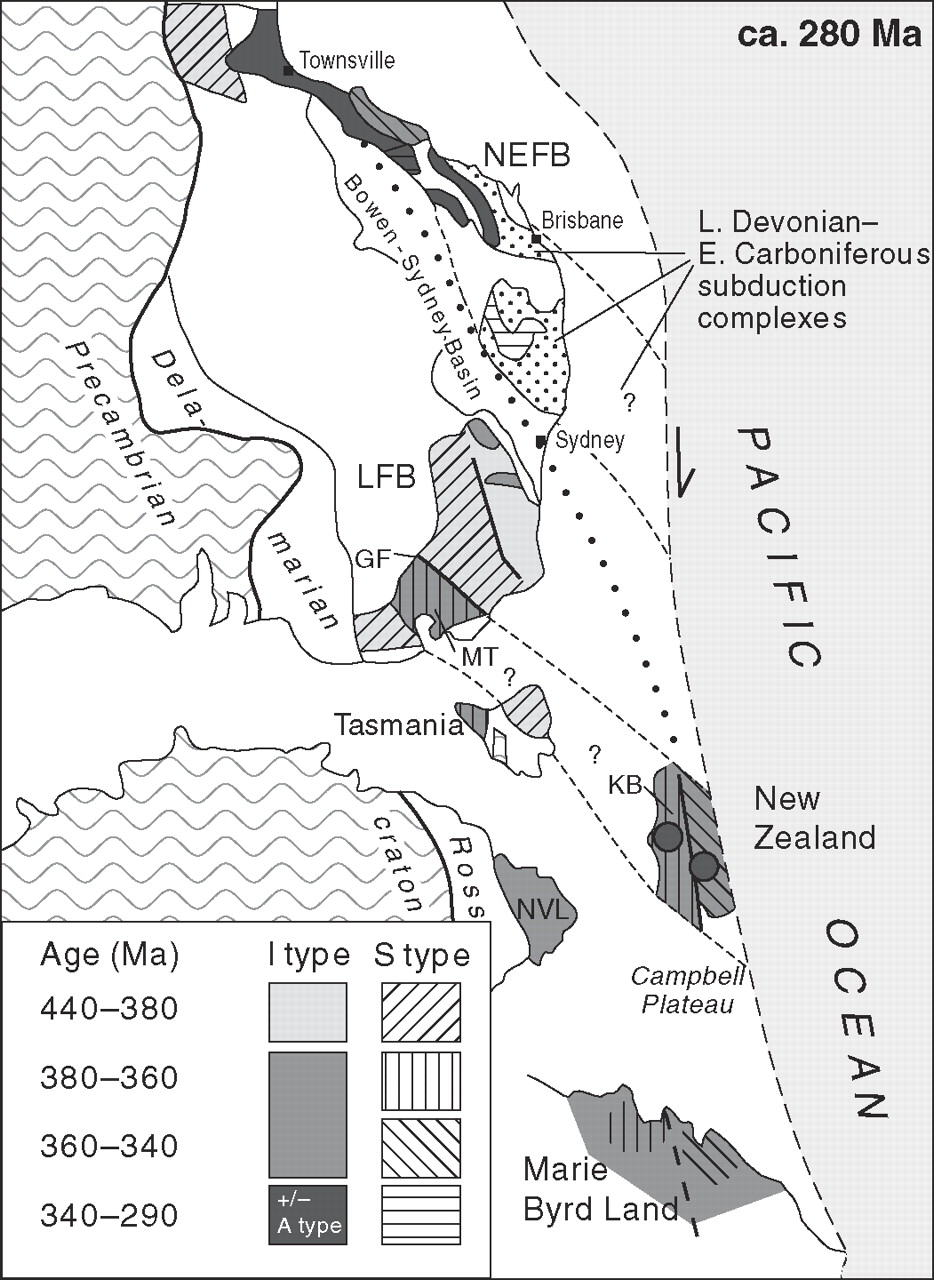
\includegraphics[width=1\textwidth]{Granite_Types_from_the_Eastern_Australian_Margin.jpg}
\caption{\label{fig:GraniteTypes}Granite Types from the Mesozoic Eastern Australian Margin}
\end{figure}

\begin{figure}
\centering
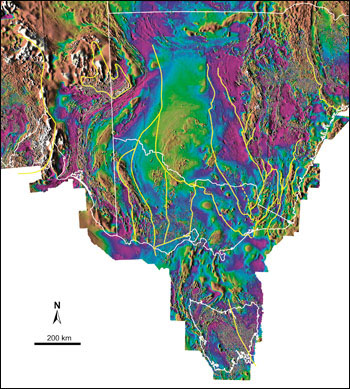
\includegraphics[width=1\textwidth]{Geology_Neoproterozoic_Fig_1.jpg}
\caption{\label{fig:mangneticImage}Regional magnetic image of southeastern Australia showing structural zone boundaries. Data sources: GSV, AGSO, PIRSA, MRT and GSNSW http://www.energyandresources.vic.gov.au/earth-resources/geology-of-victoria/geological-history/neo-car}
\end{figure}

\begin{figure}
\centering
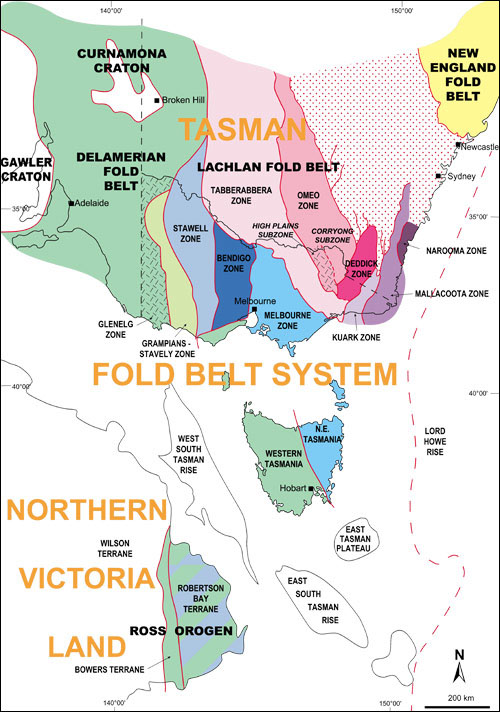
\includegraphics[width=1\textwidth]{Geology_Neoproterozoic_Fig_2.jpg}
\caption{\label{fig:
VicStructuralZones}Map of eastern Australian fold belts and Victorian structural zones http://www.energyandresources.vic.gov.au/earth-resources/geology-of-victoria/geological-history/neo-car}
\end{figure}

\begin{figure}
\centering
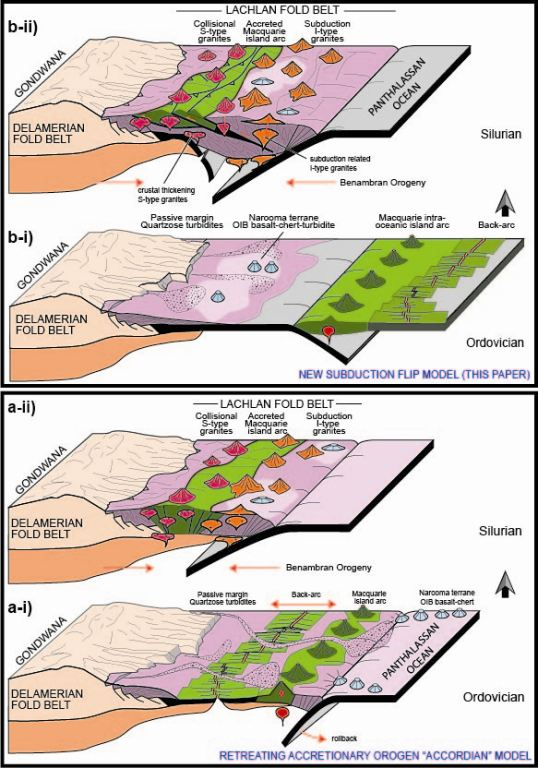
\includegraphics[width=1\textwidth]{granite_models.jpg}
\caption{\label{fig:GraniteModels} Possible formation models}
\end{figure}







\section{Conclusion}

Conclusion


\newpage

\bibliography{bibliography.bib}

\end{document}